
\section{Machine learning module}
\subsection{Dataset source}
The dataset used is gotten from \href{https://www.kaggle.com/datasets/fedesoriano/heart-failure-prediction}{kaggle} and was made by putting together different datasets that were already out there but had never been put together before. In this dataset, 5 heart datasets are put together based on 11 common features. This makes it the largest dataset for heart disease research that has been made available so far. The five datasets that were used to put it together are:
\begin{enumerate}[label=(\alph*)]
	\item Cleveland: 303 observations
	\item Hungarian: 294 observations
	\item Switzerland: 123 observations
	\item Long Beach VA: 200 observations
	\item Stalog (Heart) Data Set: 270 observations
\end{enumerate}

\comment{The classification process was carried out with the use of k-nn, naive bayes, decision tree, and logistic regression algorithms.}

\subsection{Exploratory data analysis}

\subsubsection{Correlation chart}
A correlation matrix is nothing more than a table that displays the correlation coefficients for various variables. The matrix illustrates the relationship between all possible pairings of values in a table. It is a strong tool for summarizing a large dataset as well as identifying and visualizing trends in the data.

\begin{lstlisting}[language=Python, caption={Correlation chart}]
	pd.options.display.float_format = "{:,.3f}".format
	plt.figure(figsize=(10,8))
	sns.set_context('notebook',font_scale = 1.15)
	sns.heatmap(df.corr(),annot=True, linewidths=1)
	plt.savefig("corr.png")
	plt.show()
\end{lstlisting}
\begin{figure}[htb]
	\centering
	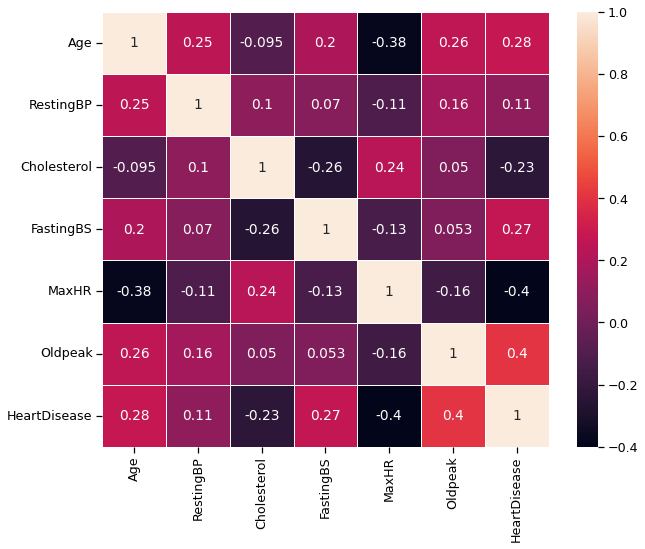
\includegraphics[scale=0.65]{correlation-chart.png}
	\caption{Correlation chart}
	\label{fig:correlation-chart}
\end{figure}
From the correlation chart \figurename~\ref{fig:correlation-chart} we can see that:
\begin{enumerate}[label=(\roman*)]
	\item{Oldpeak is highly positively correlated to the target variable.}
	\item{MaxHR is highly negatively correlated toe the target variable.}
	\item{RestingBP has the lowest correlation compared to other attributes}
\end{enumerate}
\subsubsection{Plotting numerical values}
In Listing~\ref{lst:plot-numerical} I plotted age and fasting blood sugar count with the target column.
\begin{lstlisting}[language=Python, caption={Plotting select numerical features with target column}, label={lst:plot-numerical}]
	cols_to_plot = ["Age", "FastingBS"]
	for i in cols_to_plot:
		plt.figure(figsize=(14,5))
		sns.countplot(x=df[i], data=df, hue='HeartDisease')
		plt.legend(['Normal', 'Heart Disease'])
		plt.title(i)
		plt.tight_layout()
\end{lstlisting}
\comment{
\begin{figure}[htb]
	\centering
	\begin{floatrow}
		\ffigbox[\FBwidth]{\caption{Ages chart}\label{}}{
			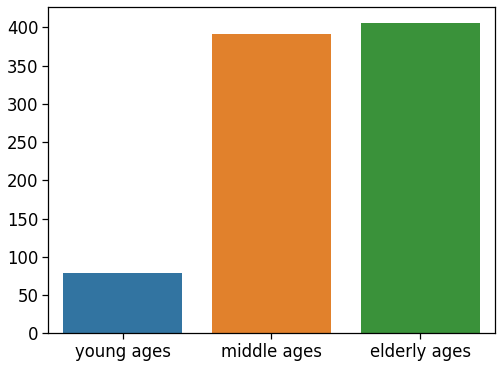
\includegraphics[scale=0.4]{ages-chart.png}}
		\ffigbox[\FBwidth]{\caption{FastingBS chart}\label{}}{
			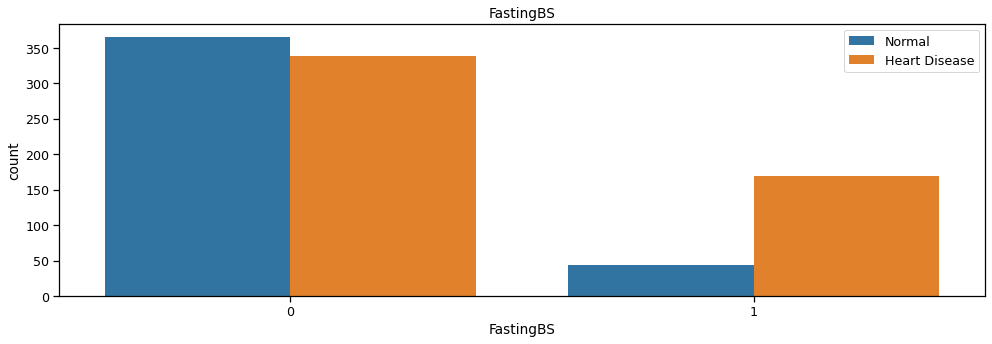
\includegraphics[width=3in, height=3in]{fasting-bs-chart.png}}
	\end{floatrow}
\end{figure}
}

\begin{figure}[htb]
	\centering
	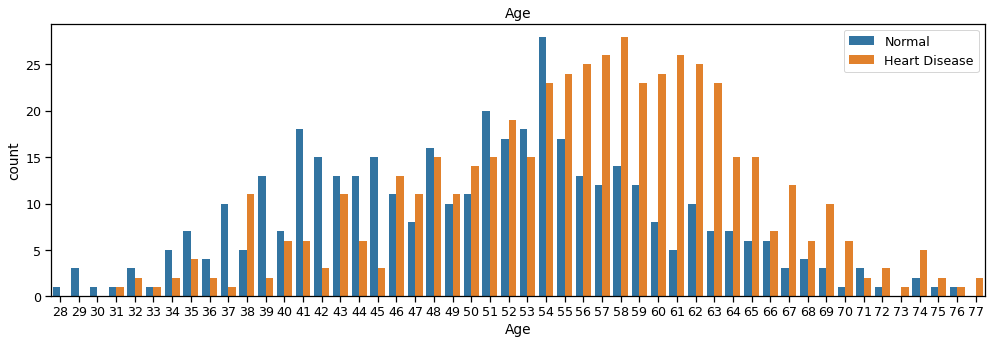
\includegraphics[scale=0.45]{age-count-chart.png}
	\caption{Age}
	\label{fig:age-count-chart}
\end{figure}
We can see that in \figurename~\ref{fig:age-count-chart} the occurrence of heart disease in the older ages from 55 to 77 is higher.

\begin{figure}[htb]
	\centering
	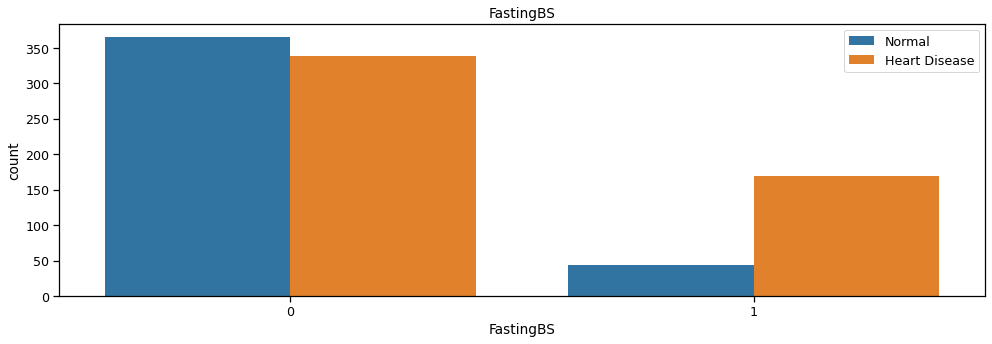
\includegraphics[scale=0.45,]{fasting-bs-chart.png}
	\caption{Fasting blood sugar}
	\label{fig:fasting-bs-chart}
\end{figure}

From the figure in ~\ref{fig:fasting-bs-chart} we can infer that higher fasting blood sugar is more likely to have heart disease.
\subsubsection{Plotting categorical values}

\begin{lstlisting}[language=Python, caption={Plotting categorical values}]
	# ploting categorical features with target
	for i in categorical:
		plt.figure(figsize=(10,5))
		sns.countplot(x=i, data=df, hue='HeartDisease', edgecolor='black')
		plt.legend(['Normal', 'Heart Disease'])
		plt.title(i)
		plt.show()
\end{lstlisting}

\begin{figure}[htb]
	\centering
	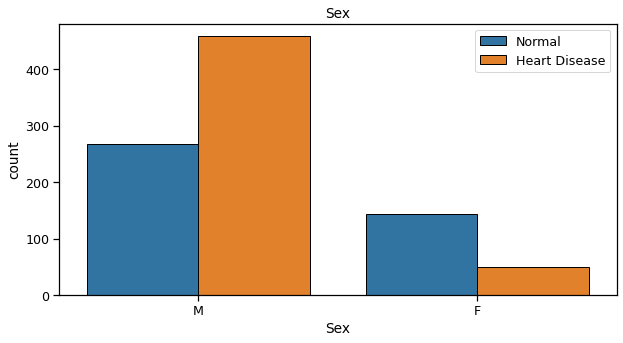
\includegraphics[scale=0.45]{sex-chart.png}
	\caption{Sex}
	\label{fig:sex-chart}
\end{figure}
\figurename~\ref{fig:sex-chart} shows that there's more occurrence of heart disease in males than females.

\begin{figure}[htb]
	\centering
	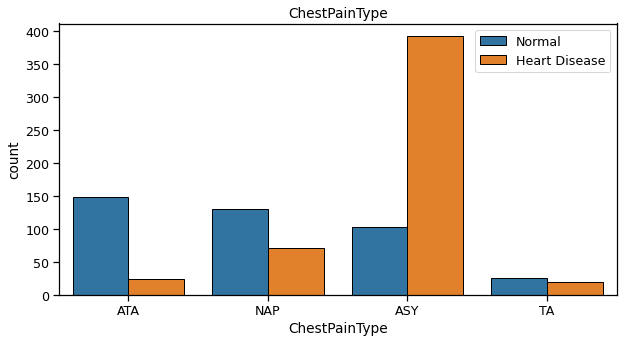
\includegraphics[scale=0.45]{chestpaintype-chart.png}
	\caption{Chest pain type}
	\label{fig:chestpaintype-chart}
\end{figure}
We can see from \figurename~\ref{fig:chestpaintype-chart} that the Asymptomatic chest pain type is highly correlated with heart disease.

\begin{figure}[htb]
	\centering
	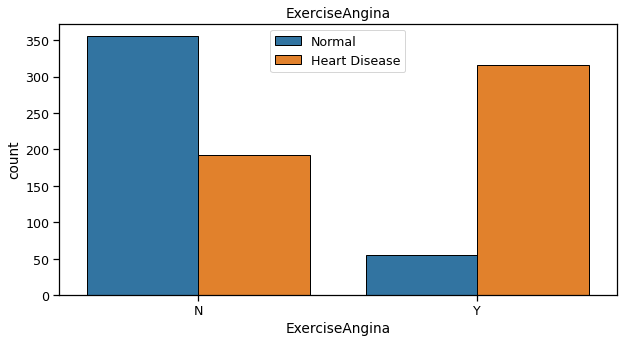
\includegraphics[scale=0.45]{exercise-angina-chart.png}
	\caption{Exercise angina}
	\label{fig:exercise-angina-chart}
\end{figure}

\begin{figure}[htb]
	\centering
	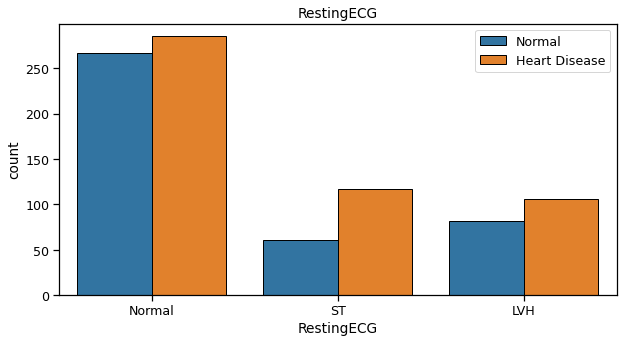
\includegraphics[scale=0.45]{restingecg-chart.png}
	\caption{Resting electrocardiogram results}
	\label{fig:restingect-chart}
\end{figure}

\subsection{Data preprocessing}
The preprocessing steps in the following subsections were applied on the dataset.
\subsubsection{Imputation}
Before imputation, we have to check for missing values in the dataset.
\begin{lstlisting}[language=Python, caption=Dataset information]
	df.info()\end{lstlisting}
Output:
\begin{lstlisting}[numbers=none]
	RangeIndex: 918 entries, 0 to 917
	Data columns (total 12 columns):
	#   Column          Non-Null Count  Dtype  
	---  ------          --------------  -----  
	0   Age             918 non-null    int64  
	1   Sex             918 non-null    object 
	2   ChestPainType   918 non-null    object 
	3   RestingBP       918 non-null    int64  
	4   Cholesterol     918 non-null    int64  
	5   FastingBS       918 non-null    int64  
	6   RestingECG      918 non-null    object 
	7   MaxHR           918 non-null    int64  
	8   ExerciseAngina  918 non-null    object 
	9   Oldpeak         918 non-null    float64
	10  ST_Slope        918 non-null    object 
	11  HeartDisease    918 non-null    int64  
	dtypes: float64(1), int64(6), object(5)
	memory usage: 86.2+ KB
\end{lstlisting}

\comment{

We can see from the output that there are no null values in the dataset. Also, The \textit{string} columns in the dataset are represented as \textit{object} and need to be converted to \textit{string} types.


\begin{lstlisting}[language=Python, caption={Convert object columns to string}]
	string_col = df.select_dtypes(include="object").columns
	df[string_col]=df[string_col].astype("string")
\end{lstlisting}
}

\subsubsection{Feature scaling}
Feature scaling was done using the MinMaxScaler class in the sklearn library on the dataframe used to train non-tree based algorithms.

\begin{lstlisting}[language=Python, caption={Scaling with MinMaxScaler}]
	from sklearn.preprocessing import MinMaxScaler
	
	scal = MinMaxScaler()
	X_train = scal.fit_transform(df_nontree[feature_col_nontree].values)
	Y_train = df_nontree[target_col]
	df[string_col]=df[string_col].astype("string")
\end{lstlisting}

\subsubsection{Handling of categorical values}
Label encoding is used in this study to encoding is used for Decision tree model while One-Hot encoder is used for the non-tree based algorithms.

\begin{lstlisting}[language=Python, caption={Applying Label Encoder to the dataframe}]
	from sklearn.preprocessing import LabelEncoder
	
	le = LabelEncoder()
	df_cat = df[string_col].apply(le.fit_transform)
\end{lstlisting}

\begin{lstlisting}[language=Python, caption={Applying One-Hot Encoder to the dataframe}]
	from sklearn.preprocessing import OneHotEncoder
	from sklearn.compose import make_column_transformer
	
	target_col="HeartDisease"
	
	
	df_nontree = df.drop(target_col,axis=1)
	
	ohe = OneHotEncoder(handle_unknown='ignore')
	
	transformer = make_column_transformer(
		(OneHotEncoder(), string_col),
		remainder='passthrough',
		verbose_feature_names_out=False
	)
	
	transformed = transformer.fit_transform(df_nontree)
		df_nontree = pd.DataFrame(
		transformed, 
		columns=transformer.get_feature_names_out()
	)
\end{lstlisting}

\subsection{Training and Performance analysis}
The dataset was split using StratifiedKFold over 5 folds for cross validation and the accuracy of every fold was calculated using area under the ROC curve (AUC) to get precision, recall and f1-score.


\subsubsection{Logistic Regression}
Logistic regression had a peak accuracy of 88\% after cross-validation

\subsubsection{Naive Bayes}
Naive Bayes had a peak accuracy of 88.3\% after cross-validation

\subsubsection{KNN}
K-nearest neighbours had a peak accuracy of 91.6\% after cross-validation

\subsubsection{Decision Tree}
Decision Tree had a peak accuracy of 77.2\% after cross-validation

\section{Web Server module}
The web server contains the views and the inference engine. The views module is responsible for responding to http request from a client. The home page displays a form \figurename~\ref{fig:site-2} for the user to enter the medical data. When the data form is sent, the server processes the data and returns the results and inference in the result page, \figurename~\ref{fig:site-3}

\begin{lstlisting}[language=Python, caption={app.py}, label={lst:app.py}]
	from flask import Flask
	from flask_assets import Bundle, Environment
	from app.views.index import index
	from app.config import Config
	
	def create_app():
		app = Flask(__name__)
		app.config.from_object(Config)
		assets = Environment(app)
		
		css = Bundle("src/main.css", output="dist/main.css")
		
		assets.register("css", css)
		css.build()
		
		app.register_blueprint(index)
		
		return app
\end{lstlisting}

\begin{figure}[htb]
	\centering
	\makebox[0cm]{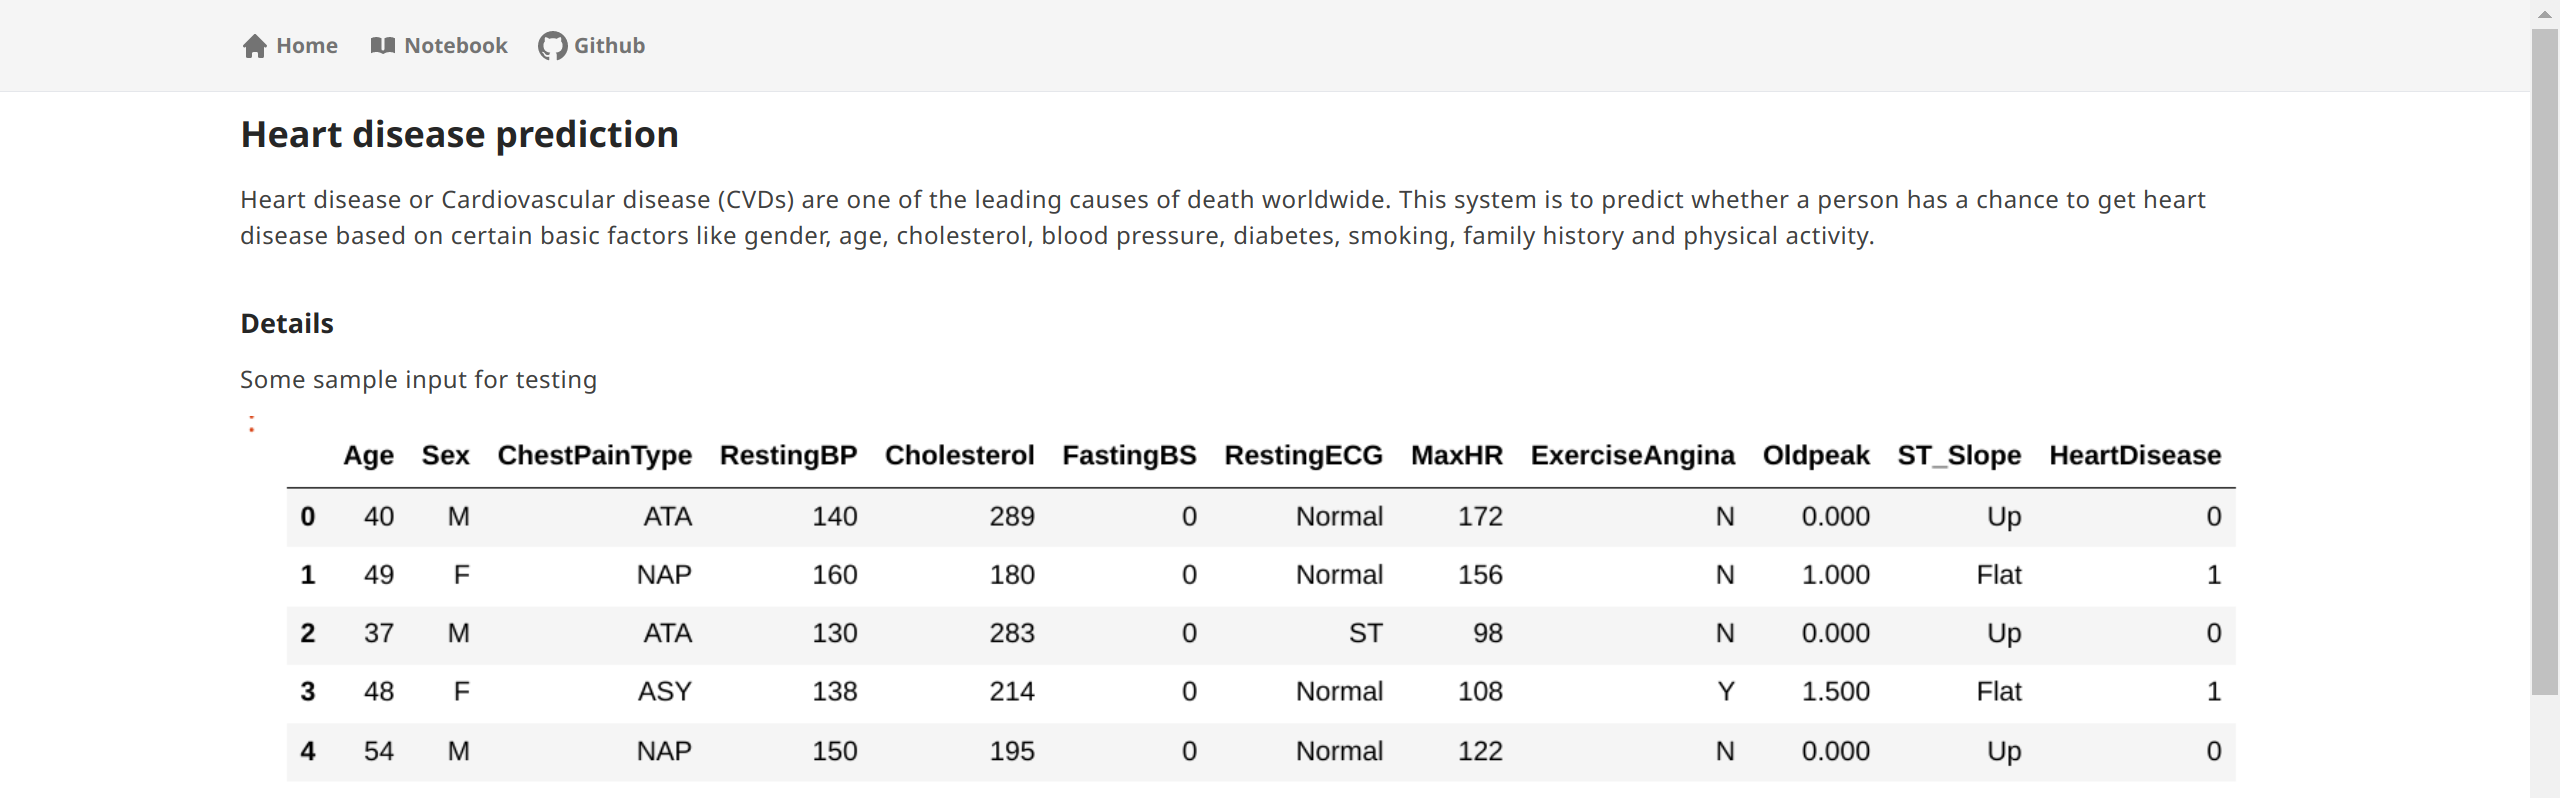
\includegraphics[scale=0.5]{site-1.png}}
	\caption{Webpage top}
	\label{fig:site-1}
\end{figure}

\begin{figure}[htb]
	\centering
	\makebox[0cm]{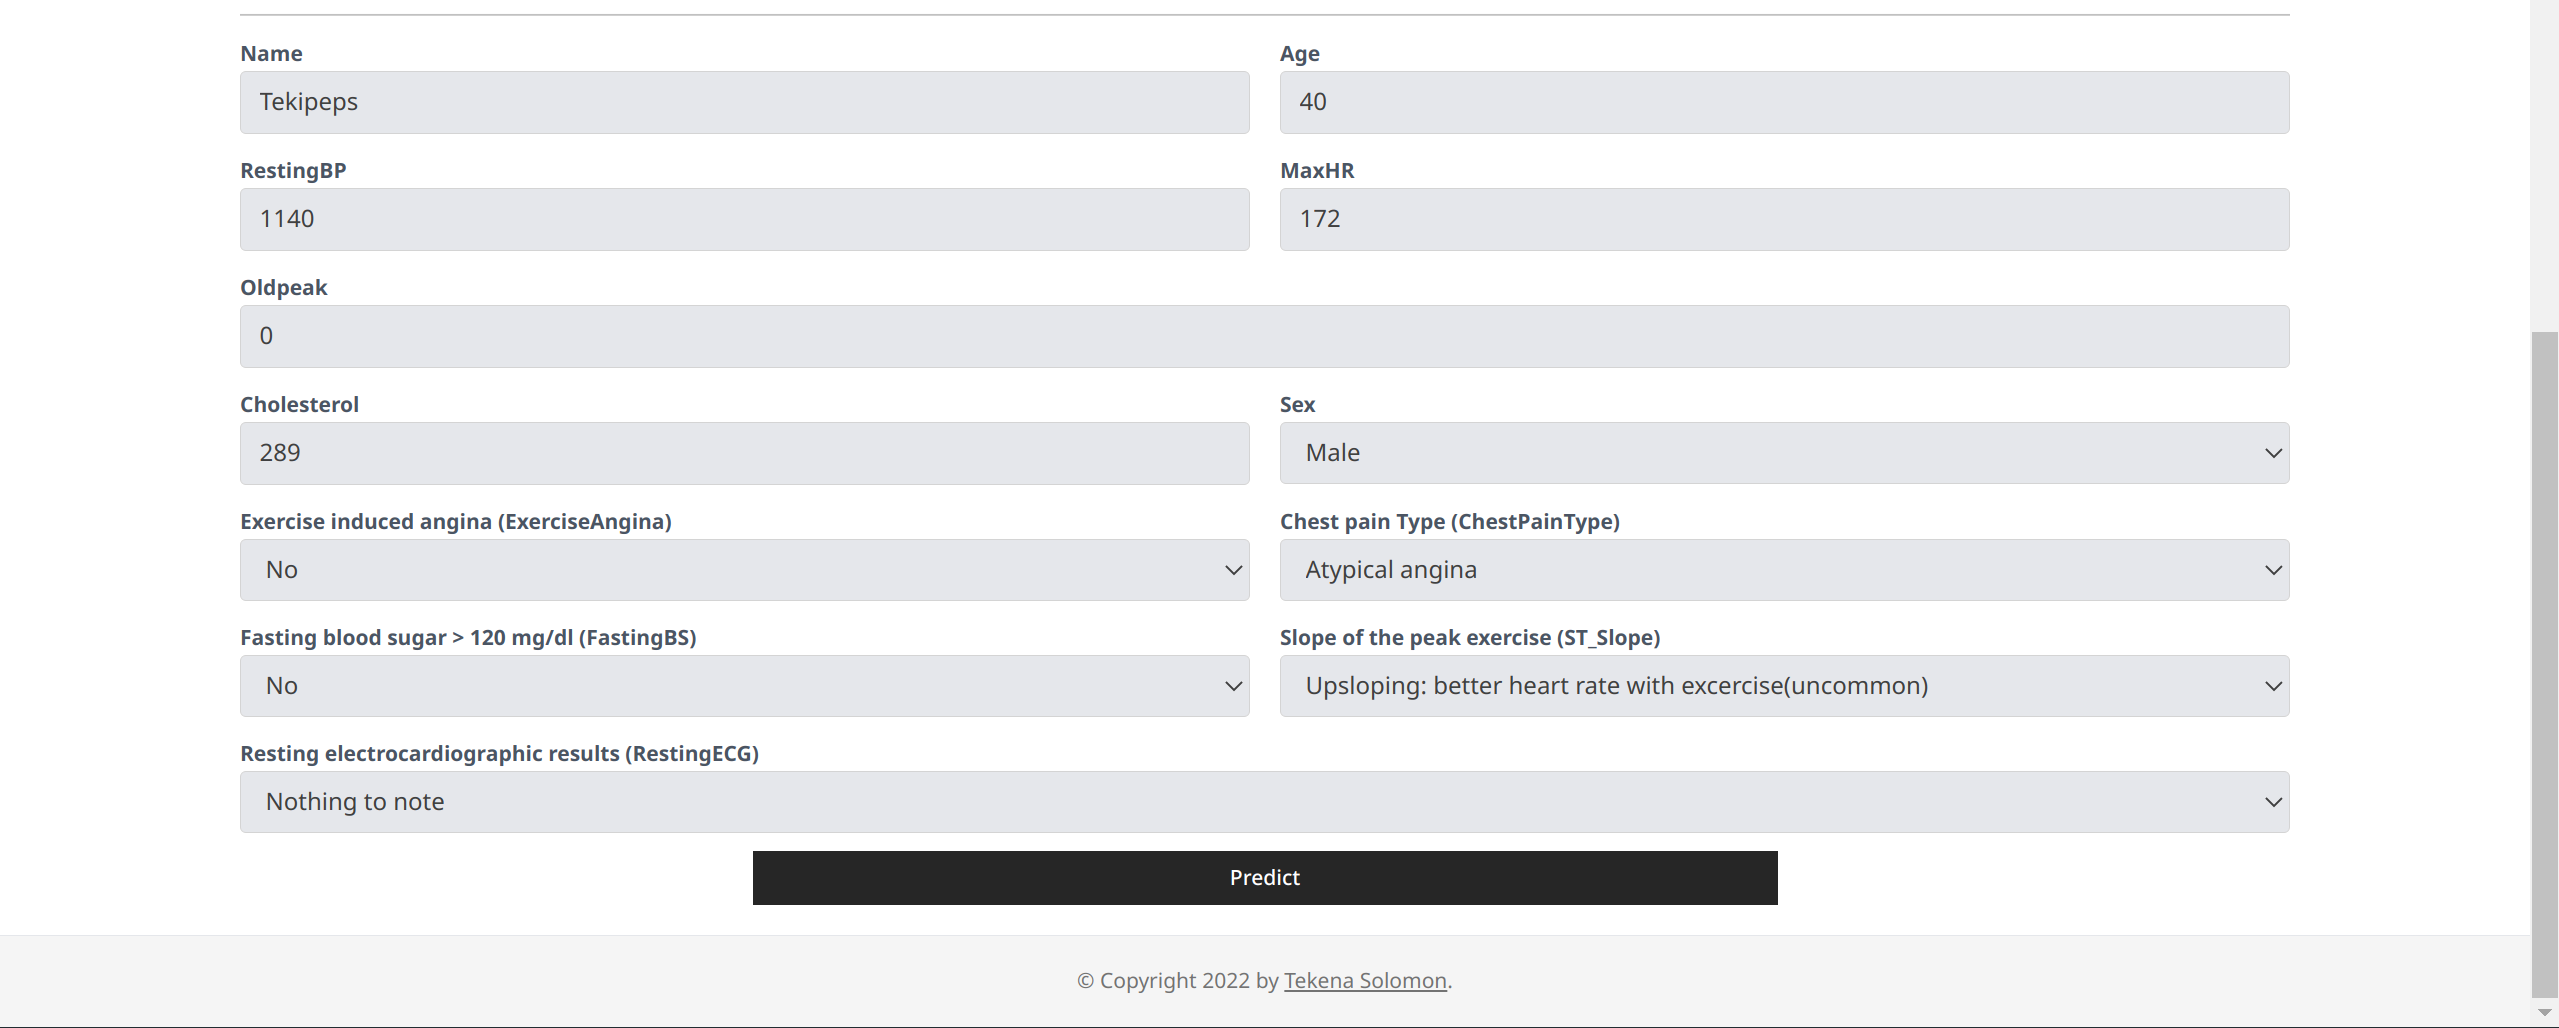
\includegraphics[scale=0.5]{site-2.png}}
	\caption{Webpage form}
	\label{fig:site-2}
\end{figure}
\begin{figure}[htb]
	\centering
	\makebox[0cm]{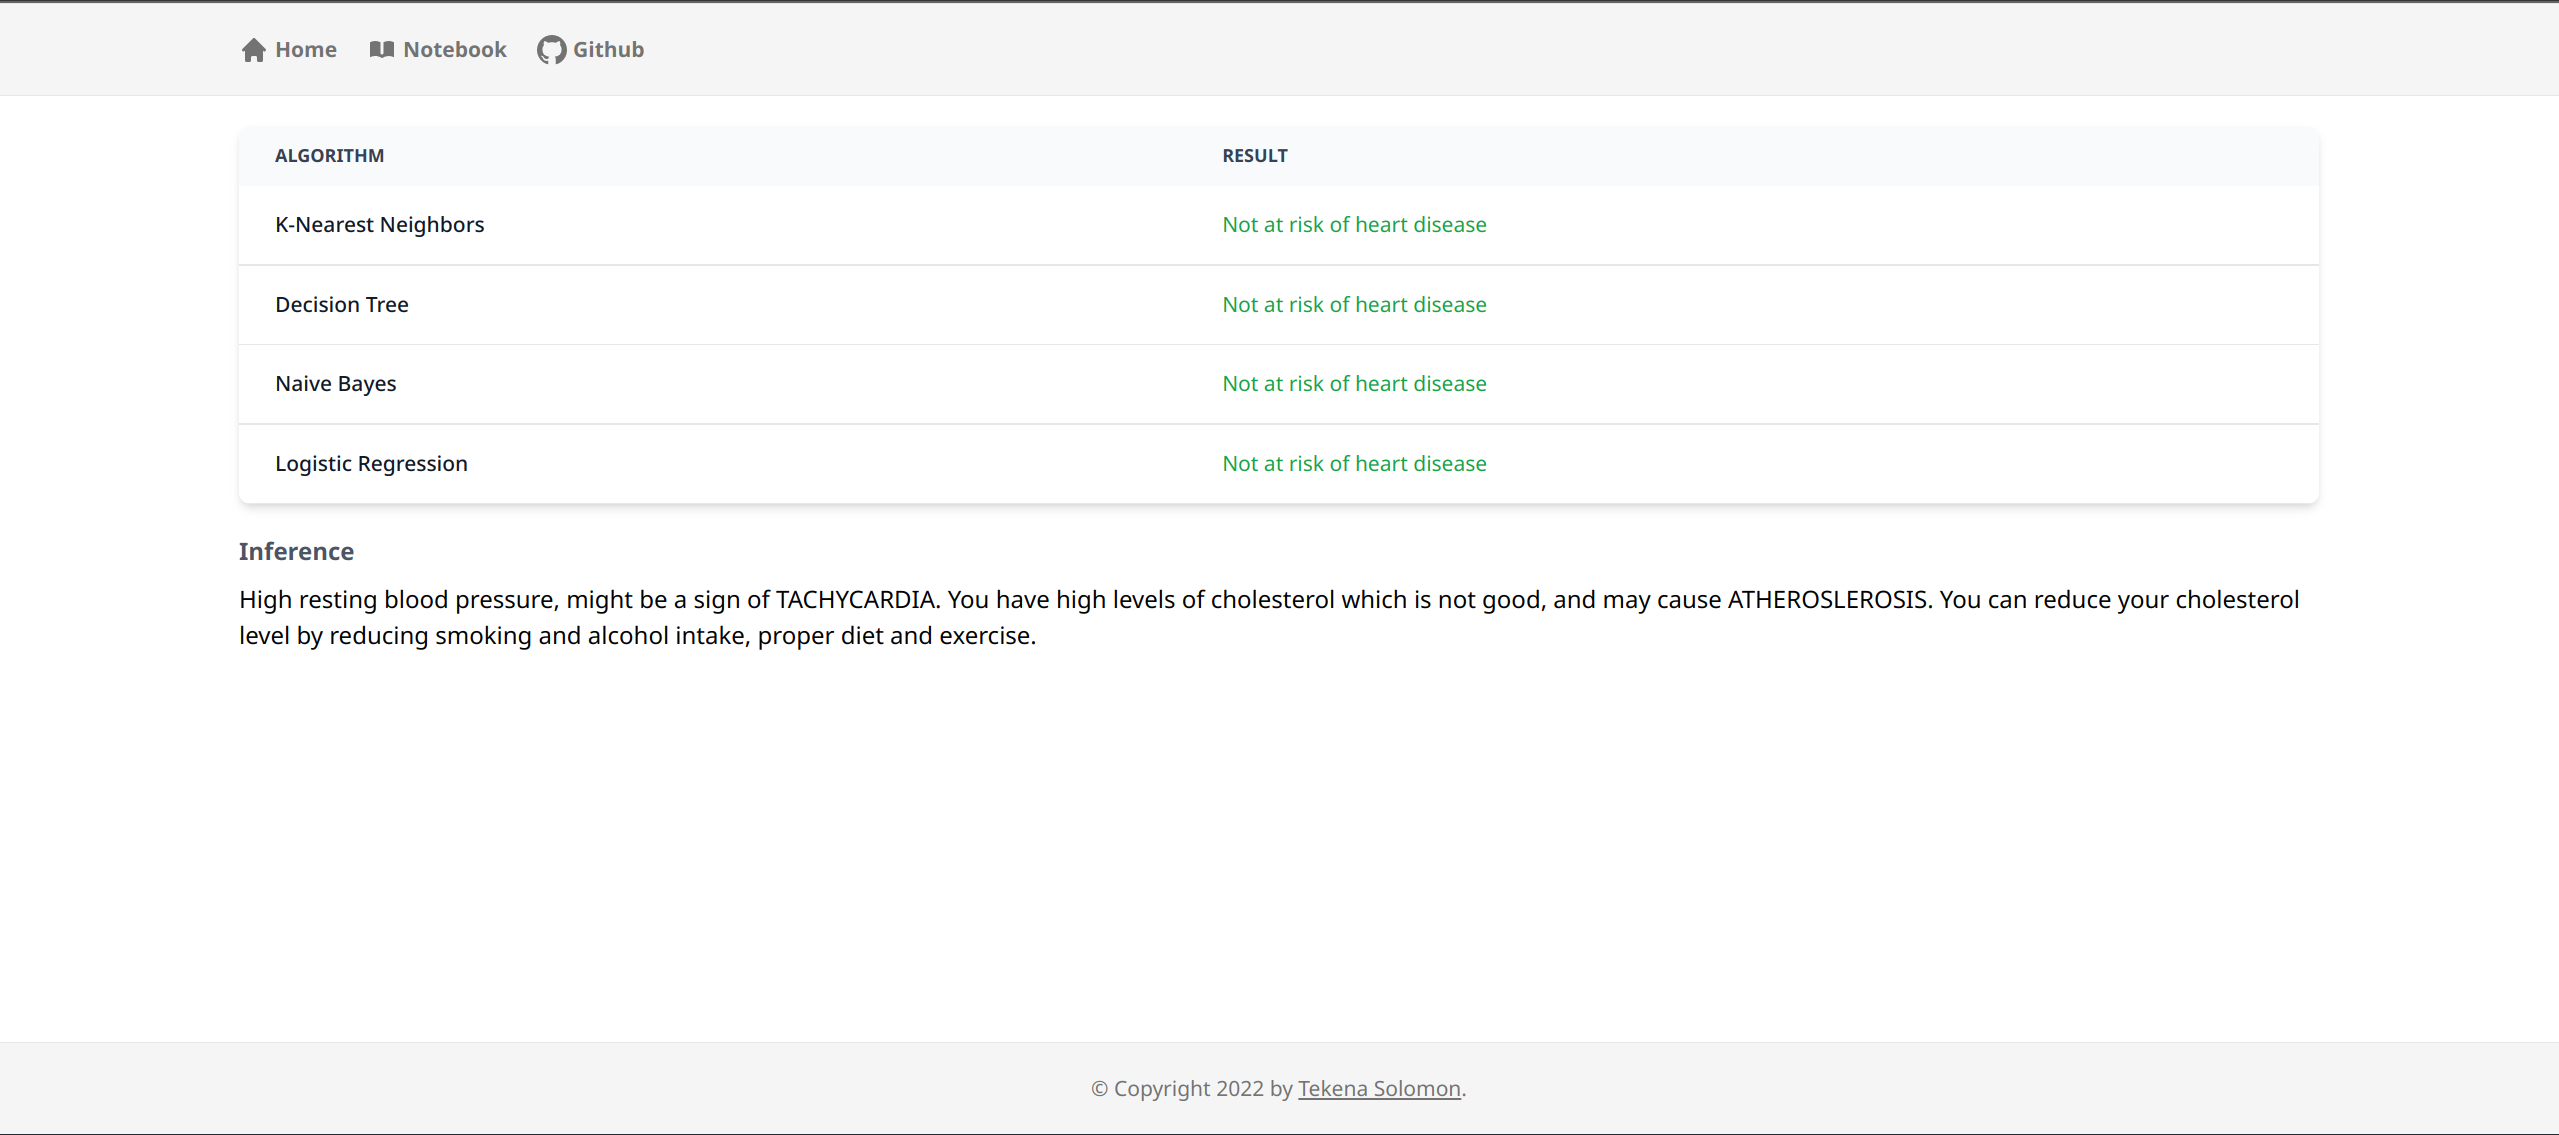
\includegraphics[scale=0.5]{site-3.png}}
	\caption{Results page}
	\label{fig:site-3}
\end{figure}



\section{Inference engine module}
The inference engine module is responsible for producing inference on the medical data. It consists of the knowledge base and the parser.

\subsection{Knowledge base}
The knowledge base is encoded in yaml format. It contains the attributes and conditions (rules) on those attributes that produce an inference.

\begin{figure}[htb]
	\centering
	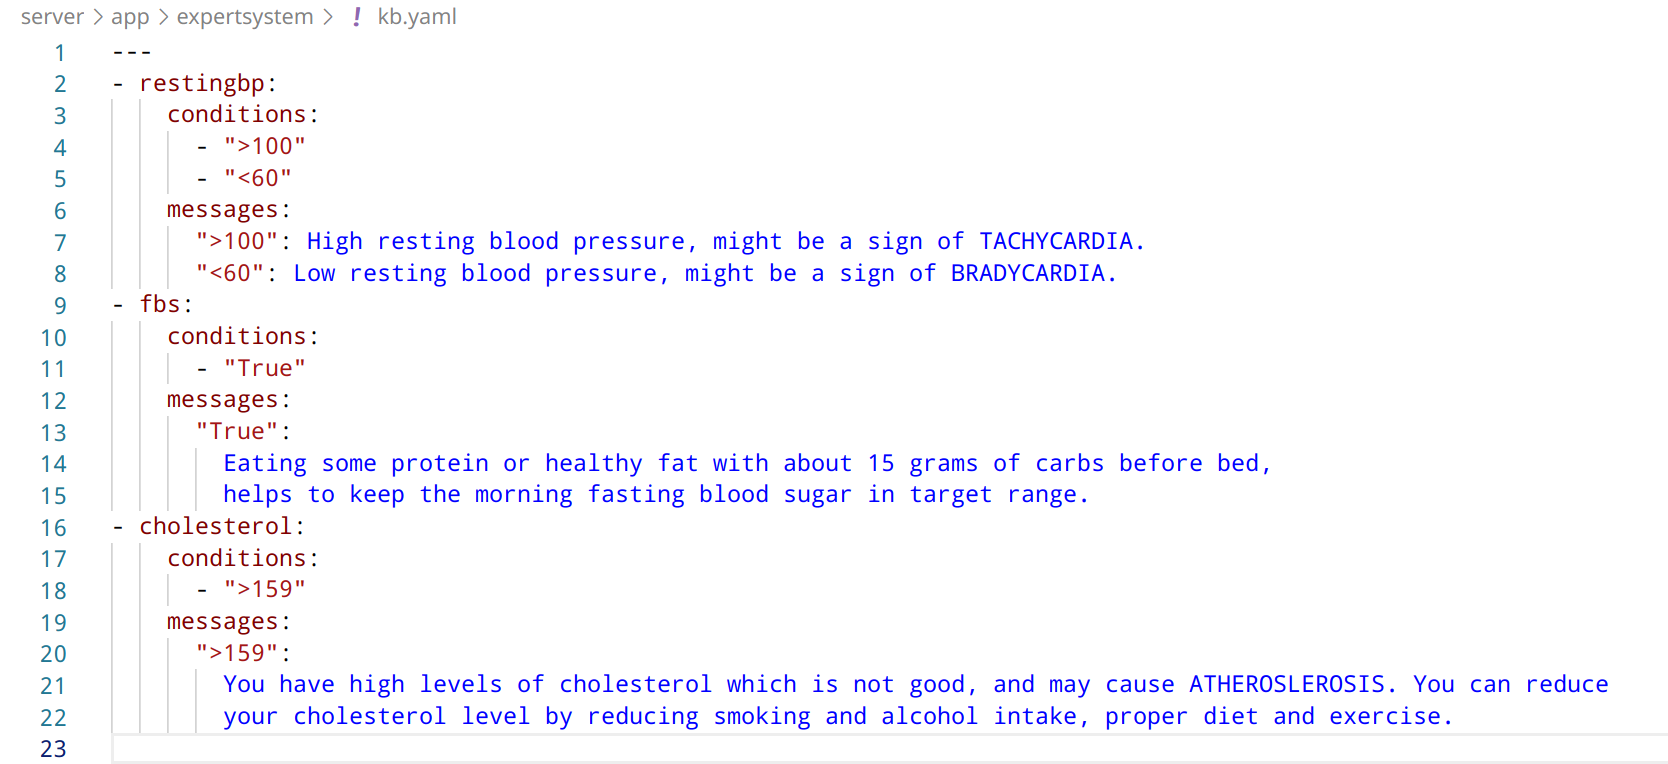
\includegraphics[scale=0.67]{kb.png}
	\caption{Knowledge base}
	\label{fig:kb}
\end{figure}

\subsection{Parser}
The parser parses the knowledge base and provides output based on the medical data. The parser takes the medical data as a lookup table to be able to call the values while parsing.

\begin{lstlisting}[language=Python, caption={Knowledge base parser}, numbers=none]
	def parse_conditions(kb, table):
		inference = ""
		for attribute in kb:
			attrname = list(attribute.keys())[0]
			for condition in attribute[attrname]["conditions"]:
				if condition.startswith(">"):
					val = int(condition[1:])
					if table[attrname] > val:
						inference += attribute[attrname]["messages"][condition] + " "
				elif condition.startswith("<"):
					val = int(condition[1:])
					if table[attrname] < val:
						inference += attribute[attrname]["messages"][condition] + " "
				elif condition == "True":
					if table[attrname] == True:
						inference += attribute[attrname]["messages"][condition] + " "
				elif condition == "False":
					if table[attrname] == False:
						inference += attribute[attrname]["messages"][condition] + " "
		
		return inference
	
\end{lstlisting}